\subsection{Рассматриваемая функция}
\def\steps{1000}
\def\T{20}

Рассмотрим прямоугольную функцию, которая задается следующим образом:
\begin{equation}
    f(t) = \begin{cases}
        1, & |t| <= 1/2, \\
        0, & |t| > 1/2
    \end{cases}
\end{equation}

Ее график приведен на рисунке \ref{fig:\steps_\T_wave_func}.
\begin{figure}[ht!]
    \centering
    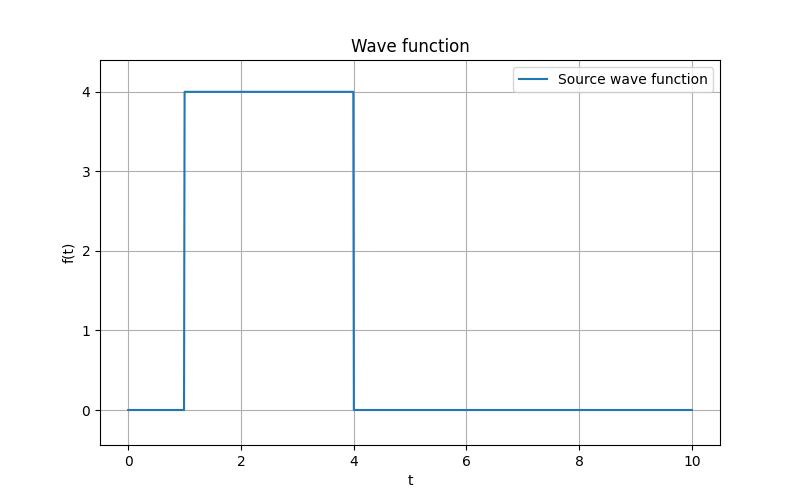
\includegraphics[width=\textwidth]{plots/\steps_\T/wave_func}
    \caption{График прямоугольной функции}
    \label{fig:\steps_\T_wave_func}
\end{figure}

\subsection{Нахождения образа аналитически}
\begin{equation}
    F(v) = \hat{f} = \int_{-\infty}^{\infty} f(t) e^{-2\pi i v t} dt = \int_{-1/2}^{1/2} e^{-2\pi i v t} dt = \frac{e^{-\pi i v} - e^{\pi i v}}{-2\pi i v} = \frac{\sin(\pi v)}{\pi v} = \sinc(\pi v)
\end{equation}

График истинного образа функции приведен на рисунке \ref{fig:\steps_\T_true_image}.
\begin{figure}[ht!]
    \centering
    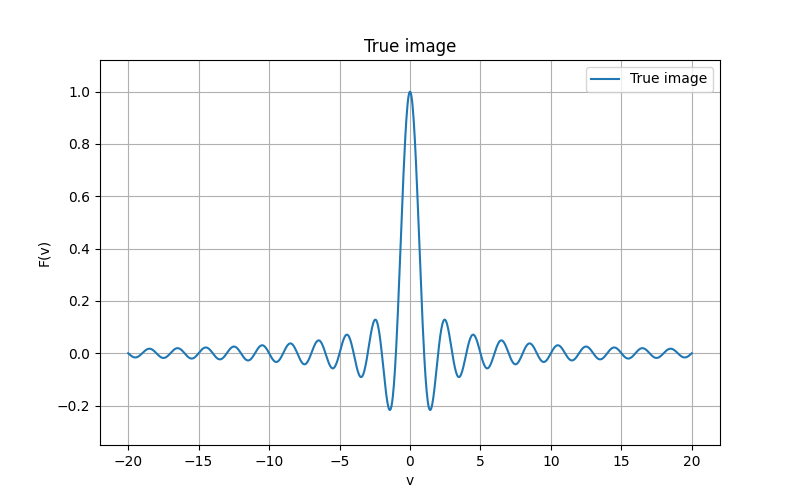
\includegraphics[width=\textwidth]{plots/\steps_\T/true_image}
    \caption{Истинный образ функции}
    \label{fig:\steps_\T_true_image}
\end{figure}

\subsection{Нахождение образа численно}
Теперь, для того, чтобы найти образ данной функции, воспользуемся численным интегрированием. 
Так как такой метод не может обеспечить интегрирование по бесконечному интервалу, то будем интегрировать по ограниченному интервалу.
Для начала рассмотрим разбиение из $\steps$ точек и интегрирование по интервалу $[-\T, \T]$.

График образа функции $f(t)$, полученный численным методом, приведен на рисунке \ref{fig:\steps_\T_num_image}.
\begin{figure}[ht!]
    \centering
    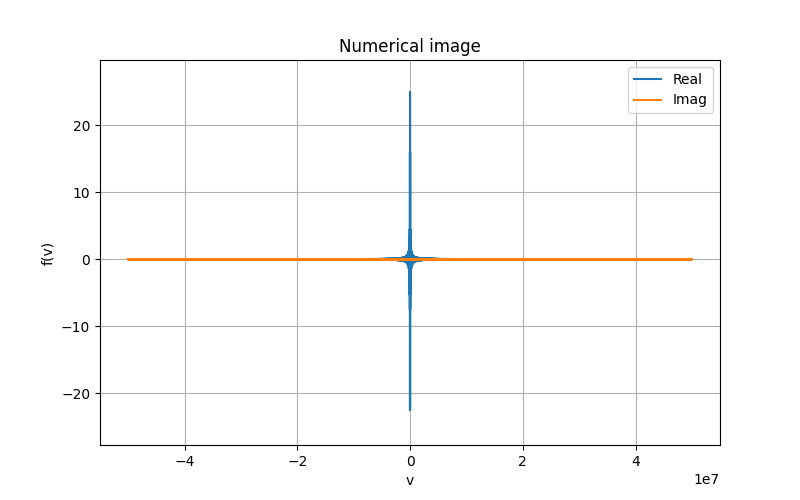
\includegraphics[width=\textwidth]{plots/\steps_\T/num_image}
    \caption{Образ функции, полученный численным методом (разбиение на $\steps$ точек, интервал $[-\T, \T]$)}
    \label{fig:\steps_\T_num_image}
\end{figure}

Рассмотрим сравнительный график истинного и численного образа функции на рисунке \ref{fig:\steps_\T_cmp_images}.
\begin{figure}[ht!]
    \centering
    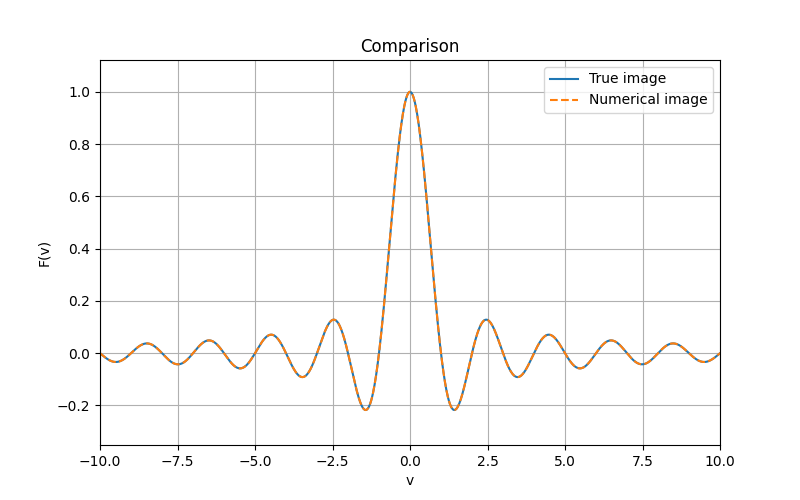
\includegraphics[width=\textwidth]{plots/\steps_\T/cmp_images}
    \caption{Сравнение истинного и численного образа функции (разбиение на $\steps$ точек, интервал $[-\T, \T]$)}
    \label{fig:\steps_\T_cmp_images}
\end{figure}

Графики истинного и численного образа функции совпадают, что говорит о корректности
численного метода. Для более подробного анализа рассмотрим графики разности истинного и
численного образа функции \textit{(ошибки)} на рисунке \ref{fig:\steps_\T_error}.
\begin{figure}[ht!]
    \centering
    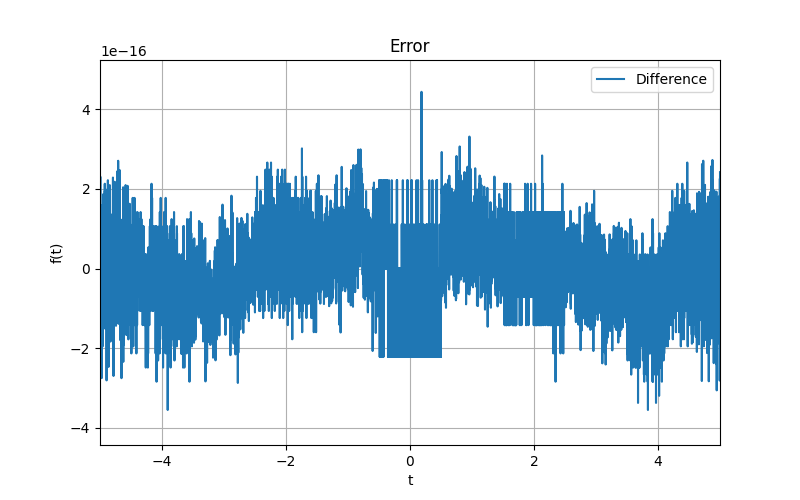
\includegraphics[width=\textwidth]{plots/\steps_\T/error}
    \caption{График ошибки (разбиение на $\steps$ точек, интервал $[-\T, \T]$)}
    \label{fig:\steps_\T_error}
\end{figure}
На рисунке \ref{fig:\steps_\T_error} видно, что ошибка представляет из себя гармоническую функцию
с амплитудой $\approx 10^{-3}$, что говорит о том, что численный метод хорошо смог приблизиться к истинному образу функции.

\subsection{Восстановление функции}
Теперь, имея образ функции, можно восстановить исходную функцию. Применим обратное преобразование Фурье к численному образу функции 
и сравним результат с исходной функцией. Графики исходной функции и восстановленной функции приведены на рисунке \ref{fig:\steps_\T_cmp_restored}.
\begin{figure}[ht!]
    \centering
    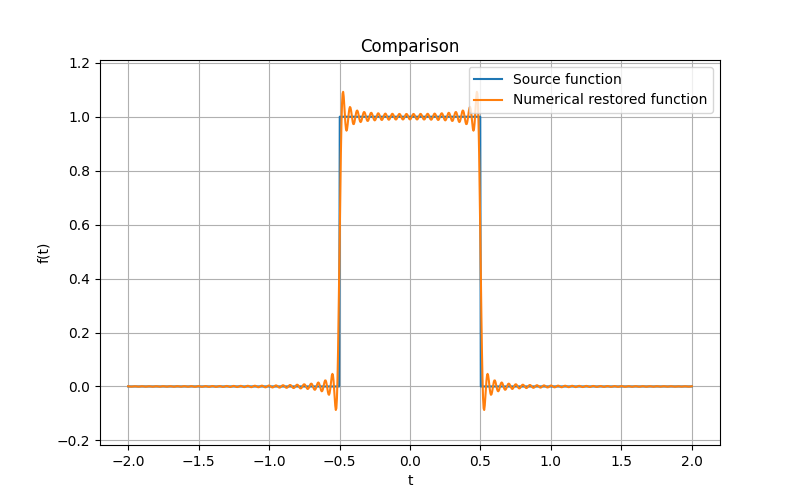
\includegraphics[width=\textwidth]{plots/\steps_\T/cmp_restored}
    \caption{Сравнение исходной и восстановленной функции (разбиение на $\steps$ точек, интервал $[-\T, \T]$)}
    \label{fig:\steps_\T_cmp_restored}
\end{figure}
На рисунке \ref{fig:\steps_\T_cmp_restored} видно, что исходная и восстановленная функции не полностью совпадают, в точках разрыва 
заметны наиболее сильные отклонения. Это связано, по большей части, с тем, что интегрирование численными методами невозможно провести на 
бесконечном интервале, а также с тем, что восстановление функции происходит с использованием образа функции, который также был получен численным методом.

\subsection{Увеличение промежутка интегрирования}
\def\steps{1000}
\def\T{80}
Для того, чтобы уменьшить ошибку восстановления функции, увеличим промежуток интегрирования до $[-\T, \T]$. Количество точек разбиения оставим прежним.

Для анализа сразу рассмотрим график ошибки на рисунке \ref{fig:\steps_\T_error}.
\begin{figure}[ht!]
    \centering
    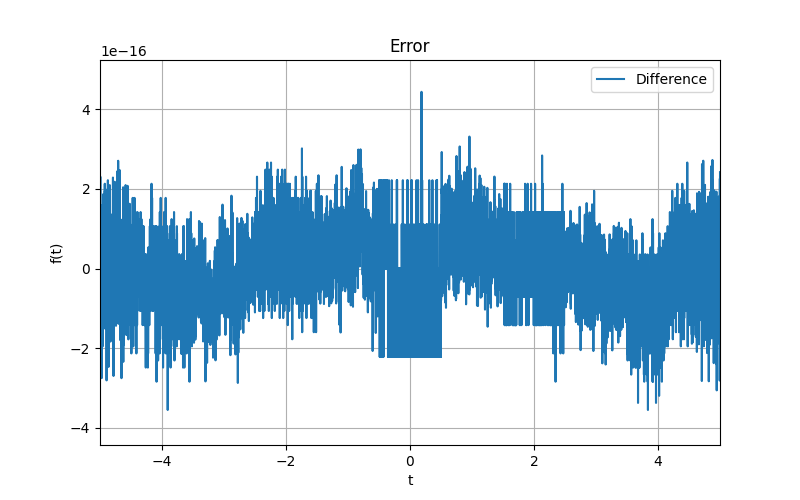
\includegraphics[width=\textwidth]{plots/\steps_\T/error}
    \caption{График ошибки (разбиение на $\steps$ точек, интервал $[-\T, \T]$)}
    \label{fig:\steps_\T_error}
\end{figure}

Ошибка, как ни странно, выросла. Это может быть связано с тем, что точность вычисления интеграла при увеличении промежутка 
интегрирования, при этом с прежним количеством точек разбиения, уменьшается. Тем не менее, рассмотрим сравнительные графики 
исходной и восстановленной функции на рисунке \ref{fig:\steps_\T_cmp_restored}.
\begin{figure}[ht!]
    \centering
    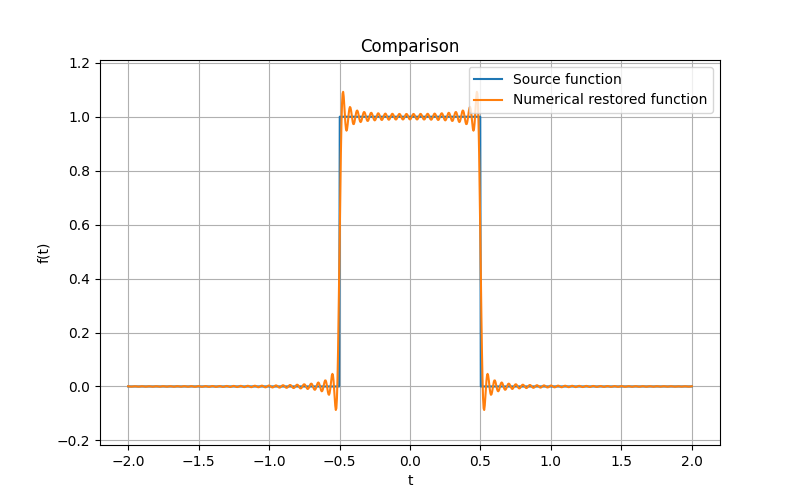
\includegraphics[width=\textwidth]{plots/\steps_\T/cmp_restored}
    \caption{Сравнение исходной и восстановленной функции (разбиение на $\steps$ точек, интервал $[-\T, \T]$)}
    \label{fig:\steps_\T_cmp_restored}
\end{figure}

На рисунке \ref{fig:\steps_\T_cmp_restored} видно, что восстановленная функция стала более похожа на исходную, чем в предыдущем случае, 
несмотря на то, что ошибка в образе функции увеличилась. Это можно связать с тем, что вклад ошибки от малого количества 
точек разбиения меньше, чем вклад ошибки от малого промежутка интегрирования функции $\sinc(\pi v)$, которая, 
хоть и стремится к нулю на бесконечности, но не равна ему на конечных интервалах.

\subsection{Увеличение количества точек разбиения}
\def\steps{10000}
\def\T{80}
Теперь, кроме увеличения промежутка интегрирования, увеличим количество точек разбиения до $\steps$. Сражу же перейдем 
к анализу графика ошибки на рисунке \ref{fig:\steps_\T_error}.
\begin{figure}[ht!]
    \centering
    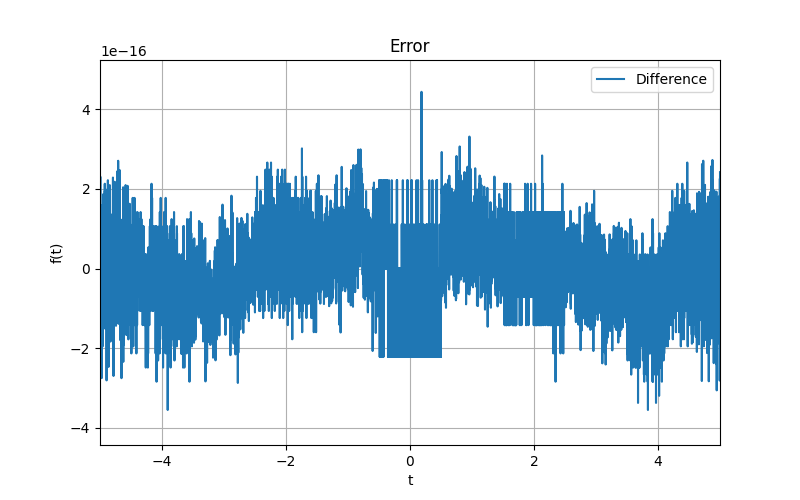
\includegraphics[width=\textwidth]{plots/\steps_\T/error}
    \caption{График ошибки (разбиение на $\steps$ точек, интервал $[-\T, \T]$)}
    \label{fig:\steps_\T_error}
\end{figure}

Ошибка уменьшилась, что говорит о том, что увеличение количества точек разбиения дает более точное интегрирование, как и предполагалось.
Теперь ошибка по модулю не превышает $10^{-4}$: при увеличении числа точек разбиения на порядок, ошибка уменьшилась на порядок.

При этом, при увеличении количества точек разбиения, сильно увеличивается время вычисления образа функции. Это, очевидно, 
связано с необходимостью проведения большего числа операций с плавающей точкой. 

Рассмотрим сравнительные графики исходной и восстановленной функции на рисунке \ref{fig:\steps_\T_cmp_restored}.
\begin{figure}[ht!]
    \centering
    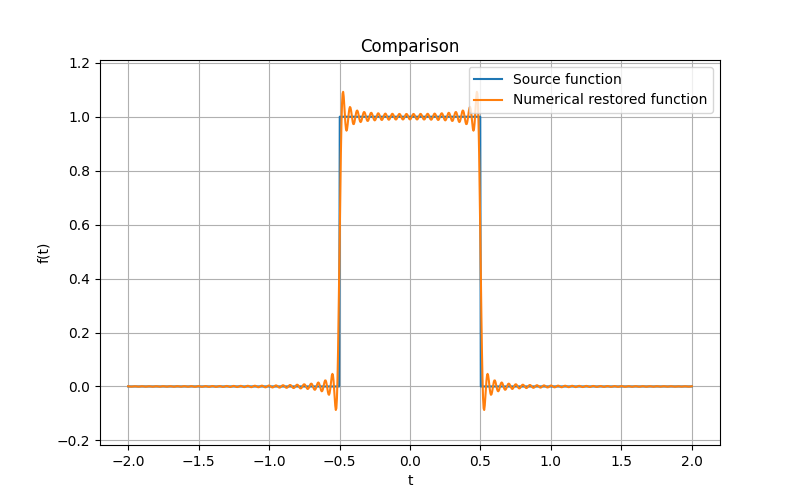
\includegraphics[width=\textwidth]{plots/\steps_\T/cmp_restored}
    \caption{Сравнение исходной и восстановленной функции (разбиение на $\steps$ точек, интервал $[-\T, \T]$)}
    \label{fig:\steps_\T_cmp_restored}
\end{figure}

В данном случае уже довольно трудно судить о величине ошибки, поэтому рассмотрим график разности исходной и восстановленной функции на рисунке \ref{fig:\steps_\T_func_error}. 
\begin{figure}[ht!]
    \centering
    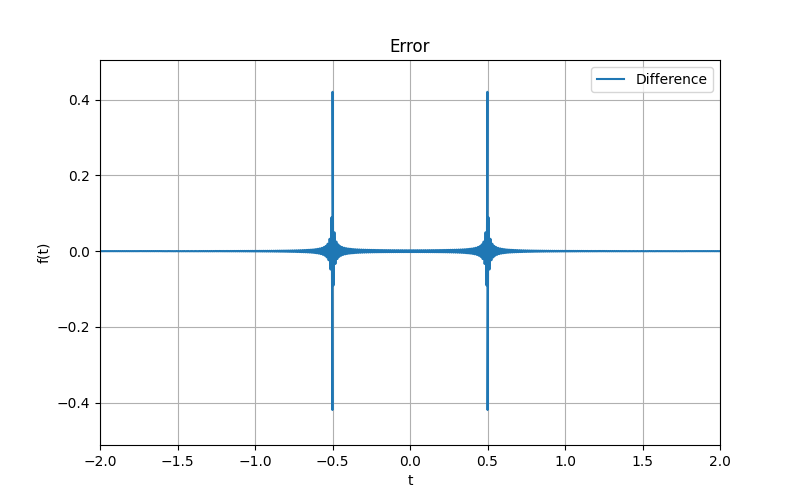
\includegraphics[width=\textwidth]{plots/\steps_\T/error_restored}
    \caption{График разности исходной и восстановленной функции (разбиение на $\steps$ точек, интервал $[-\T, \T]$)}
    \label{fig:\steps_\T_func_error}
\end{figure}

И ошибки для прошлого случая на рисунке \ref{fig:\steps_\T_error}.
\def\steps{1000}
\def\T{80}
\begin{figure}[ht!]
    \centering
    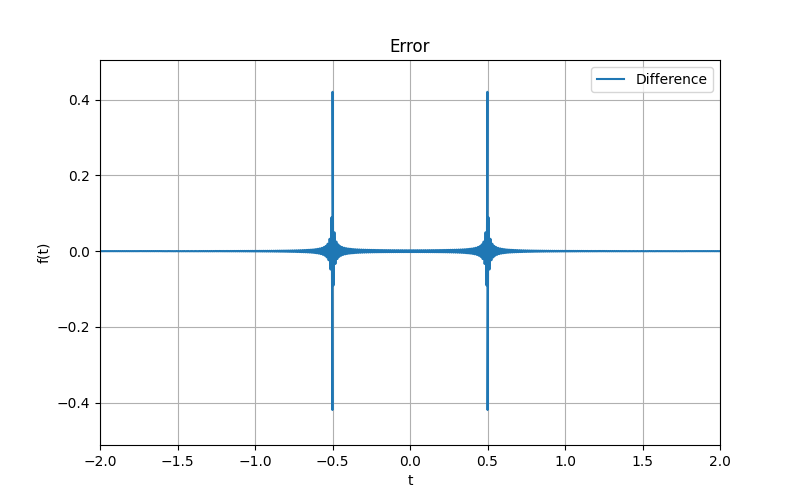
\includegraphics[width=\textwidth]{plots/\steps_\T/error_restored}
    \caption{График разности исходной и восстановленной функции (разбиение на $\steps$ точек, интервал $[-\T, \T]$)}
    \label{fig:\steps_\T_func_error}
\end{figure}

Видно, что как по величине, так и по форме, ошибка восстановления функции уменьшилась. Это говорит о том, что увеличение количества точек разбиения
дает более точное восстановление функции, что и ожидалось. 